\chapter{Implementasi dan Pengujian}
\label{chap:implementasidanpengujian}

Bab ini terdiri atas dua bagian, yaitu Implementasi Perangkat Lunak dan Pengujian Perangkat Lunak. Bagian implementasi berisi penjelasan lingkungan pengembangan perangkat lunak dan hasil implementasi. Sedangkan bagian pengujian berisi hasil pengujian perangkat lunak yang telah dibangun.

\section{Implementasi}
\label{sec:implementasi}

\subsection{Lingkungan Implementasi}
\label{subsec:lingkunganimplementasi}

Implementasi perangkat lunak ini dilakukan di sebuah komputer peneliti untuk keperluan pengujian dan penarikan kesimpulan. Komputer tersebut memiliki spesifikasi sebagai berikut :

\begin{enumerate}
	\item Processor : 1.3GHz
	\item RAM: 4.00 GB DDR3
	\item Sistem Operasi: Windows 10 Home 64-bit
	\item Versi Java : 1.8.0\_92
	\item Koneksi Internet : \textit{bandwidth up to} 1,2MBps
	\item Versi Microsoft Excel : 2016
\end{enumerate}

\subsection{Implementasi Kode Program}
\label{subsec:implementasikodeprogram}

Kode program pada perangkat lunak ditulis dalam bahasa pemrograman Java. Penulisan kode program dibagi menjadi tiga \textit{package} yaitu :\textit{Module}, \textit{Controller} dan \textit{View}. Tujuan penulisan program dibagi menjadi tiga \textit{package} adalah untuk memudahkan proses debuging. Didalam \textit{package Module} merupakan kode-kode program yang menjalankan semua fungsi mulai dari \textit{request} sampai penyimpanan file. Untuk kode program yang ada pada \textit{package Controller} merupakan kode program yang berfungsi untuk menjembatani antara tampilan dengan fungsi-fungsi untuk menjalankan perangkat lunak. Tampilan perangkat lunak ditulis didalam \textit{package View} agar dapat mendukung interaksi antarmuka agar interaksi aplikasi lebih interaktif. Penulisan kode program menggunakan \textit{library} : jsoup dengan versi 1.10.1, JSON dengan versi 20160810 dan swingx-all dengan versi 1.6.4. Untuk kode-kode program tersebut dapat dilihat pada lampiran \ref{chap:kodeprogramA}, lampiran \ref{chap:kodeprogramB} dan lampiran \ref{chap:kodeprogramC}.

\subsection{Tampilan antarmuka}
\label{subsec:tampilanantarmuka}

Berikut ini merupakan hasil implementasi antarmuka untuk perangkat lunak analisis waktu tempuh kota Bandung. Pada Gambar \ref{fig:implementasiantarmukautama} merupakan tampilan utama dari perangkat lunak yang memiliki tiga jenis input sesuai dengan \ref{fig:antarmukautama} yaitu : \textit{textfield}, \textit{datepicker}, \textit{check box}. Terdapat 1 buah tombol \textit{save} yang digunakan untuk melakukan ekstraksi data dan penyimpanan data.

\begin{figure}[H]
				\centering		
				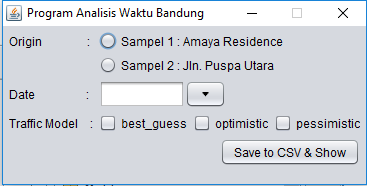
\includegraphics[scale=0.7]{Gambar/gui1.png}
				\caption[Implementasi Antarmuka Utama]{Implementasi Antarmuka Utama}
				\label{fig:implementasiantarmukautama}	
			\end{figure}
			
Pada Gambar \ref{fig:implementasifilechooser} merupakan tampilan \textit{file chooser} dari perangkat lunak yang memiliki satu buah \textit{window} untuk memilih \textit{directory} penyimpanan file. Terdapat satu buah input untuk memberi nama file. Selain itu tampilan juga terdapat filter file untuk menyimpan data dengan suatu ekstensi tertentu. Terdapat dua buah tombol untuk fitur penyimpanan yaitu : \textit{save} dimana tombol ini berfungsi untuk mengeksekusi penyimpanan file kemudian membuka file tersebut dengan aplikasi Microsoft Excel dan \textit{cancel} untuk membatalkan penyimpanan file.

\begin{figure}[H]
				\centering		
				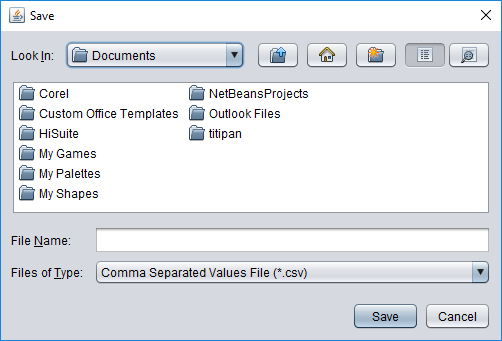
\includegraphics[scale=0.7]{Gambar/gui2.png}
				\caption[Implementasi \textit{file chooser}]{Implementasi \textit{file chooser}}
				\label{fig:implementasifilechooser}	
			\end{figure}

Pada Gambar \ref{fig:implementasihasil1}, \ref{fig:implementasihasil2} dan \ref{fig:implementasihasil3} merupakan tampilan hasil dari perangkat lunak yang memiliki satu buah tombol. Pada Gambar \ref{fig:implementasihasil1} merupakan tampilan hasil dengan menggunakan satu traffic model. Pada Gambar \ref{fig:implementasihasil2} merupakan tampilan hasil dengan menggunakan dua traffic model. Pada Gambar \ref{fig:implementasihasil3} merupakan tampilan hasil dengan menggunakan tiga traffic model.

\begin{figure}[H]
				\centering		
				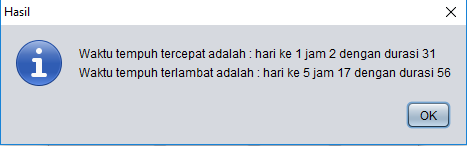
\includegraphics[scale=0.7]{Gambar/gui3.png}
				\caption[Implementasi hasil dengan satu traffic model]{Implementasi hasil dengan satu traffic model}
				\label{fig:implementasihasil1}	
			\end{figure}

\begin{figure}[H]
				\centering		
				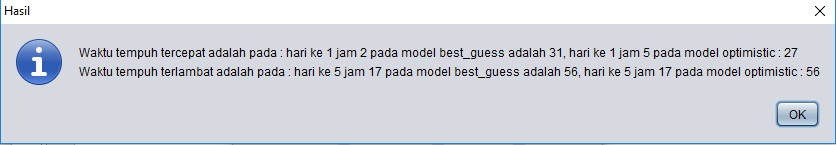
\includegraphics[scale=0.7]{Gambar/gui4.png}
				\caption[Implementasi hasil dengan dua traffic model]{Implementasi hasil dengan dua traffic model}
				\label{fig:implementasihasil2}	
			\end{figure}

\begin{figure}[H]
				\centering		
				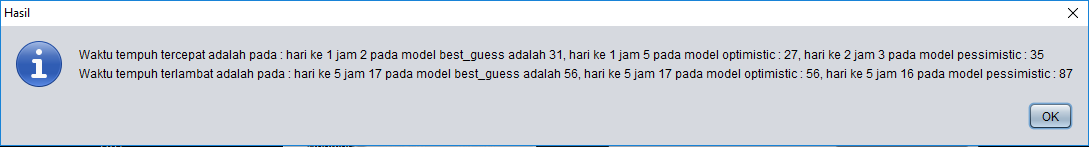
\includegraphics[scale=0.5]{Gambar/gui5.png}
				\caption[Implementasi hasil dengan tiga traffic model]{Implementasi hasil dengan tiga traffic model}
				\label{fig:implementasihasil3}	
			\end{figure}

\section{Pengujian}
\label{sec:pengujian}

\subsection{Pengujian Fungsional}
\label{subsec:pengujianfungsional}

Pengujian fungsional perangkat lunak sederhana analisis waktu tempuh kota Bandung dengan memanfaatkan Google Direction API dilakukan untuk mengetahui kesesuaian reaksi perangkat lunak dengan reaksi yang diharapkan berdasarkan aksi pengguna terhadap perangkat lunak. Pengujian ini dilakukan pada lingkungan implementasi sesuai pada subbab \ref{subsec:lingkunganimplementasi}. Terdapat 4 tes kasus yang diujikan, detail serta hasilnya dapat dilihat pada Tabel \ref{tab:pengujian1}. Beberapa data hasil ekstraksi pada pengujian ini bisa dilihat pada Lampiran \ref{chap:datahasilpengujian}. Spesifikasi pengujian fungsional adalah sebagai berikut :
\begin{enumerate}
	\item Alamat awal sampel yang digunakan adalah : Komplek Amaya Residence dan Jalan Puspa Utara.
	\item Alamat tujuan yang digunakan adalah alamat UNPAR(Universitas Katolik Parahyangan).
	\item Masukan tanggal yang digunakan adalah 17 Juli 2017 dan 24 Juli 2017.
	\item Pengujian dilakukan pada kedua sampel dengan menukar alamat awal dengan tujuan dan tidak menukar alamat awal dengan tujuan.
	\item Semua kombinasi model traffic akan digunakan untuk masing-masing mode dan masing-asing sample.
\end{enumerate}

\begin{center}
\begin{longtable}{|p{0.5cm}|p{4cm}|p{4cm}|p{4cm}|}
\hline \multicolumn{1}{|c|}\textbf{{No}} & \multicolumn{1}{c|}{\textbf{Aksi Pengguna}}& \multicolumn{1}{c|}{\textbf{Reaksi yang diharapkan}} &\multicolumn{1}{c|}{\textbf{Reaksi perangkat lunak}} \\ \hline
1 & Pengguna menjalankan program & Antarmuka utama ditampilkan & sesuai \\ \hline
2 & Pengguna memasukan longitude dan latitude, memilih tanggal, memilih ketiga model \textit{traffic} dan menekan tombol save & File berhasil disimpan dan ditampilkan dengan aplikasi microsoft excel & sesuai \\\hline
3 & Pengguna memasukan longitude dan latitude, memilih tanggal, memilih dua diantara tiga model \textit{traffic} dan menekan tombol save & File berhasil disimpan dan ditampilkan dengan aplikasi microsoft excel & sesuai \\\hline
4 & Pengguna memasukan longitude dan latitude, memilih tanggal, memilih salah satu model \textit{traffic} dan menekan tombol save & File berhasil disimpan dan ditampilkan dengan aplikasi microsoft excel & sesuai \\\hline
 &  & Jika pengguna memasukan longitude dan latitude bukan angka menampilkan pesan "Masukan angka" & sesuai \\ \hline
 &  & Jika pengguna belum memilih salah satu dari traffic\_model menampilkan pesan "Anda harus memilih minimal salah satu dari 3 traffic model yang telah disediakan" & sesuai \\\hline 
 &  & Jika pengguna belum memilih tanggal menampilkan pesan "Anda belum memilih tanggal, silahkan pilih tanggal" & sesuai \\ \hline
 &  & Jika pengguna memilih tanggal yang sudah lampau atau hari ini menampilkan pesan "Tanggal yang anda masukan adalah masa lampau atau hari ini, silahkan pilihlah tanggal yang akan datang" & sesuai \\ \hline
 &  & Jika pengguna memilih tanggal yang bukan hari senin menampilkan pesan "Tanggal yang anda pilih bukan hari senin, silahkan pilih tanggal yang merupakan hari senin" & sesuai \\ \hline
\caption{Tabel Hasil Pengujian Fungsional}
\label{tab:pengujian1}
\end{longtable}
\end{center}

\subsection{Pengujian Eksperimental}
\label{subsec:pengujianeksperimental}
Pengujian eksperimental dilakukan dengan melakukan eksperimen dari hasil ekstraksi data yang ada pada Lampiran \ref{chap:datahasilpengujian} dengan cara membuat analisis dari bagan yang datanya berasal dari hasil ekstraksi data tersebut. Pada pengujian eksperimental ini bertujuan untuk mengetahui waktu tercepat dan wakt terlambat dalam satu minggu antara dua titik yaitu : sampel dan UNPAR; UNPAR dan sampel. Dengan data yang telah diekstrak oleh program, data-data tersebut bisa dianalisis dengan bagan. Bagan itu sendiri dapat dibuat dengan memanfaatkan aplikasi Microsoft Excel secara manual. Hasil pengujian eksperimental dapat dilihat pada Lampiran \ref{chap:hasilpengujianeksperimental} yang menunjukkan perbedaan waktu tempuh pada setiap jamnya dari masing-masing sampel. Hasil pengujian eksperimental dirangkum sebagai berikut.

Pada grafik waktu masing-masing model dalam seminggu yang dapat dilihat pada Lampiran \ref{chap:hasilpengujianeksperimental}, bahwa waktu tempuh untuk setiap hari relatif memiliki waktu tempuh yang sama setiap jamnya terkecuali pada hari jumat. Pada hari jumat, waktu tempuh cenderung menurun pada pukul 12, dan lalu menaik kembali setelah itu. Hal tersebut diperkirakan oleh karena mayoritas warga indonesia beragama muslim dan melaksanakan ibadah shalat jumat pada pukul 12. Selain itu, waktu tempuh mulai menaik sejak dari pukul 6 hingga mencapai pukul 18, dan setelah itu akan selalu menurun. Waktu tempuh maksimum pada setiap harinya berada pada sekitar pukul 18. Hal tersebut diperkirakan terjadi karena pada jam tersebut merupakan saat sebagian besar orang selesai beraktifitas dan pulang ke rumah masing-masing. Sedangkan waktu tempuh yang paling minimun ada pada setiap harinya berada pada sekitar pukul 3. Hal tersebut diperkirakan terjadi karena pada jam tersebut sebagian orang masih beristirahat dirumah masing-masing.

Pengujian dilakukan dengan menukarkan alamat awal dan tujuan sesuai dengan sample. Hasil dari pengujian dengan dengan menukarkan alamat ini adalah menghasilkan bagan yang mirip dengan tidak ditukar. Tidak ada perubahan yang signifikan terhadap waktu tempuh meskipun telah ditukar alamat awal dan tujuannya.